\documentclass[../design_doc.tex]{subfiles}

\begin{document}

\section{Development Plan}\label{sec:plan}
    Development of Bookdex will span 5 weeks. A visual layout of the development plan is shown in Figure~\ref{fig:gantt}.

    To summarize the figure, there are several tasks that must be completed and each are allotted only so much time over the 5 weeks. The design document, this document, is the only task to span all 5 weeks as it will be updated as updates to other tasks occur.

    In the first week and part of the second week, much of the planning will occur. This includes diving deeper into TDS and constructing useful diagrams to better understand the required interactions between the client and server and their various states. A UML class diagram for the TDS protocol will be created so the core of the project can be observed at a glance. An additional UML class diagram will be created for the overall Bookdex application which will make use of the TDS implementation. As required, a preliminary project report will be written and submitted at the end of the first week to ensure the final goal is attainable.

    As the planning stage comes to a close in week 2, TDS implementation will begin. This will be the largest part of Bookdex but the time spent planning should accelerate the implementation. To avoid becoming bored of implementing TDS, both the client GUI and server database creation will occur in parallel. It is expected that this implementation phase will take roughly a week and a half to acheive a testable prototype.

    The remaining 2 weeks will be spent on testing and bug fixing. Of course, as issues arrise in the initial implementaiton, they will be addressed. These 2 weeks will be used to determine the limits of Bookdex.

    It is not included in Figure~\ref{fig:gantt}, but, if time permits, additional ideas outlined in the project proposal (visible in the project's \repo{Github repository}) will be added.

    At the end of the 5 weeks, Bookdex will/should be a functioning application.

    \begin{figure}
        \centering
        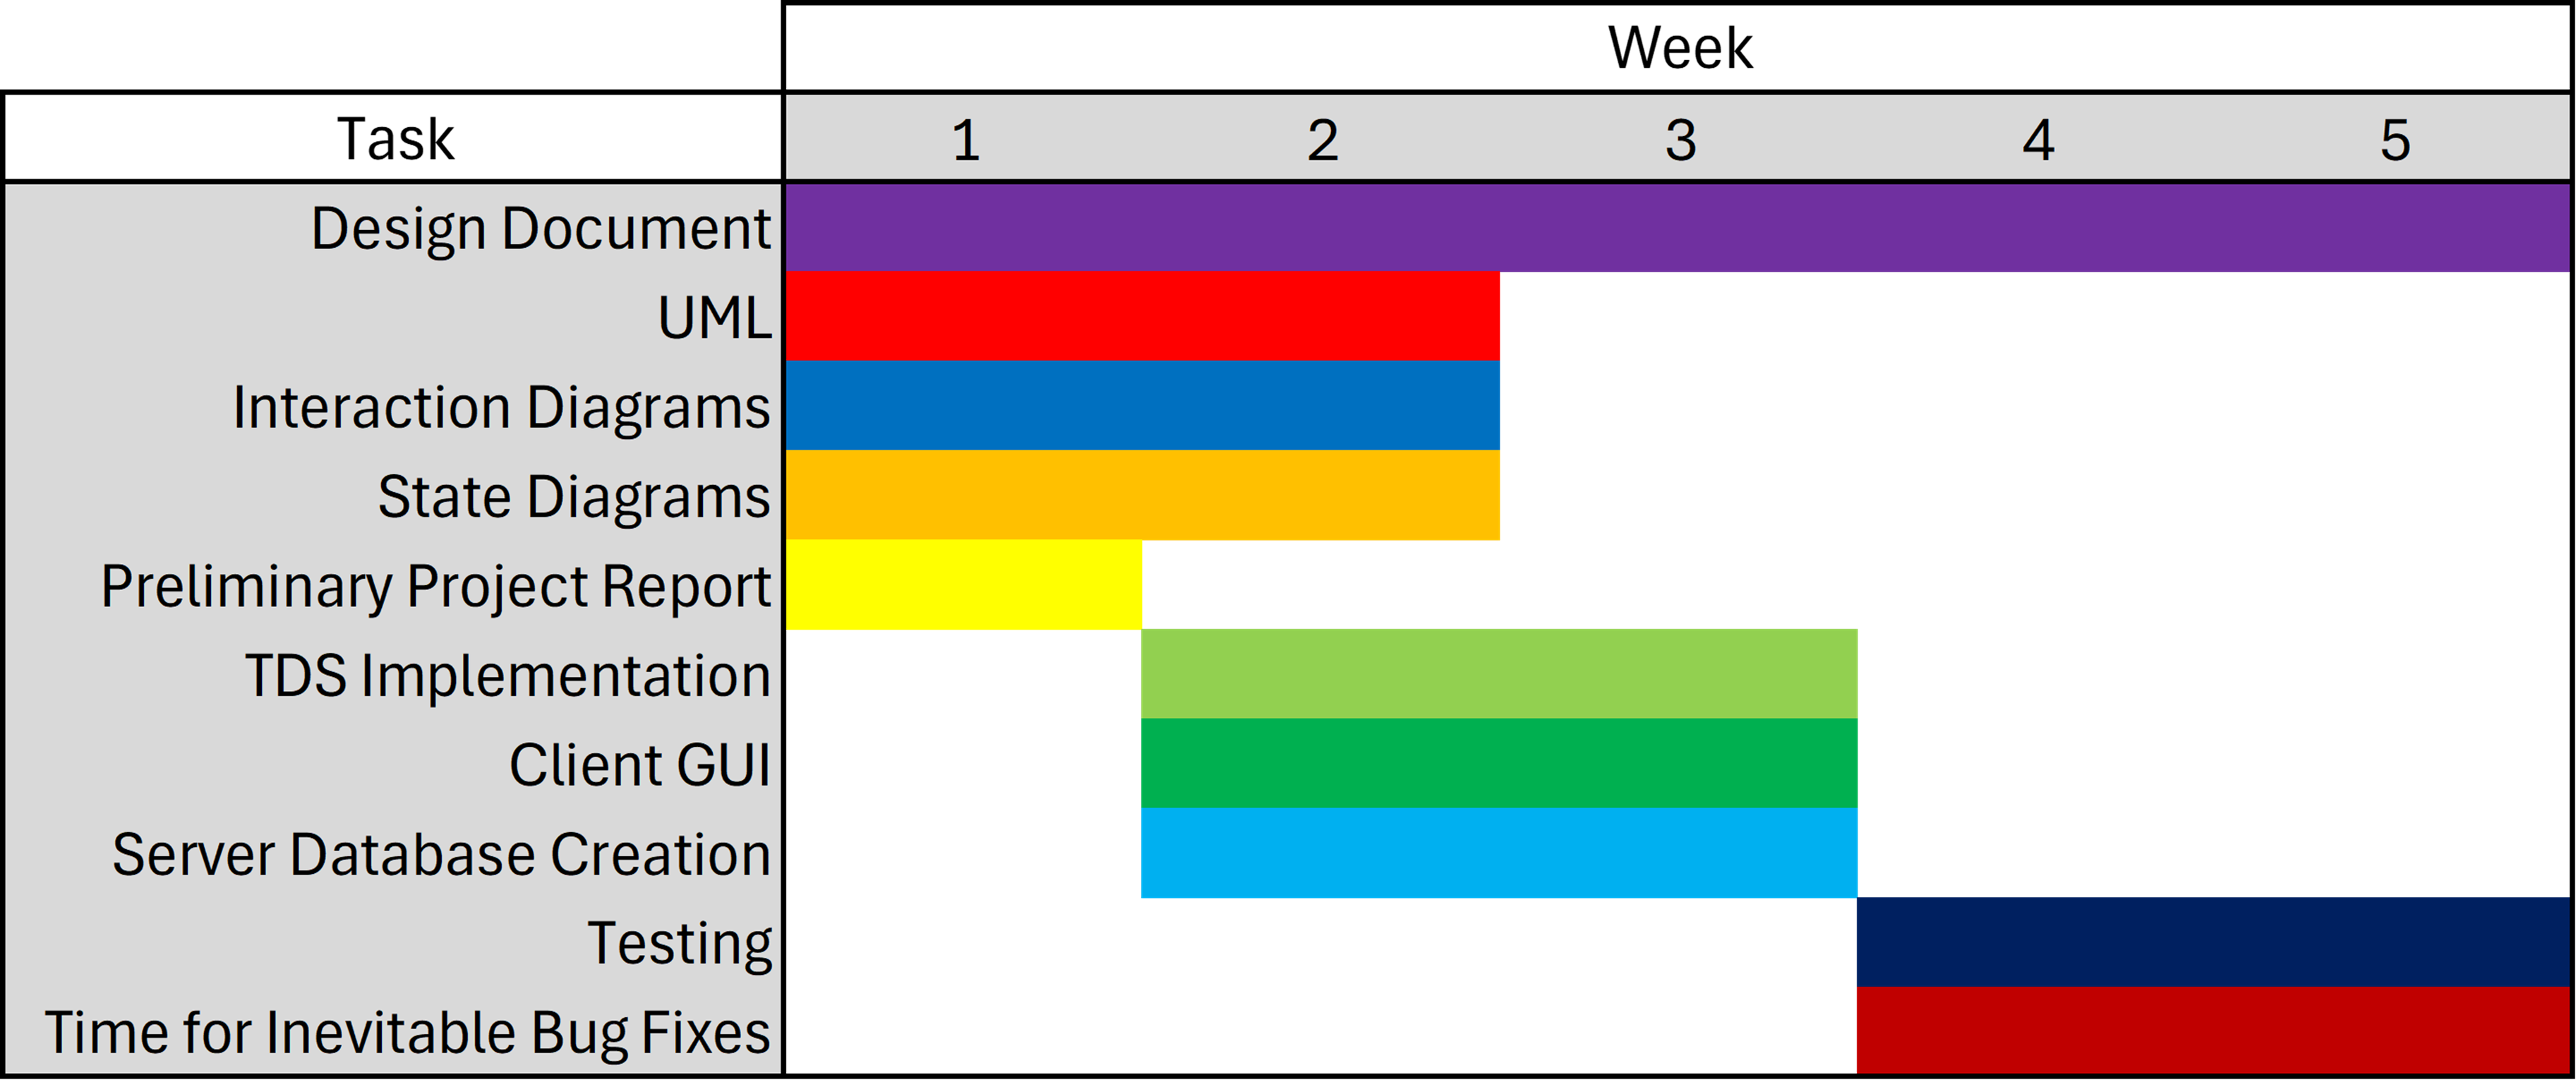
\includegraphics[width=0.9\textwidth]{gantt_chart.png}
        \caption{Gantt chart outline for the development plan for Bookdex.}\label{fig:gantt}
    \end{figure}

\end{document}